\chapter{Final System and Results}
\label{chap:final_system}

\section{Introduction}
The final Review 3 prototype is a bilingual legal and financial document assistant that accepts text-based PDFs, extracts and analyses their content, and answers questions using traceable source evidence.

\section{Final System Architecture}
The browser interface communicates with a Node.js and Express backend. The backend coordinates PDF extraction, language detection, classification, information extraction, chunking, retrieval, translation, and grounded answer generation. In-memory storage is used in the prototype.

\begin{figure}[H]
\centering
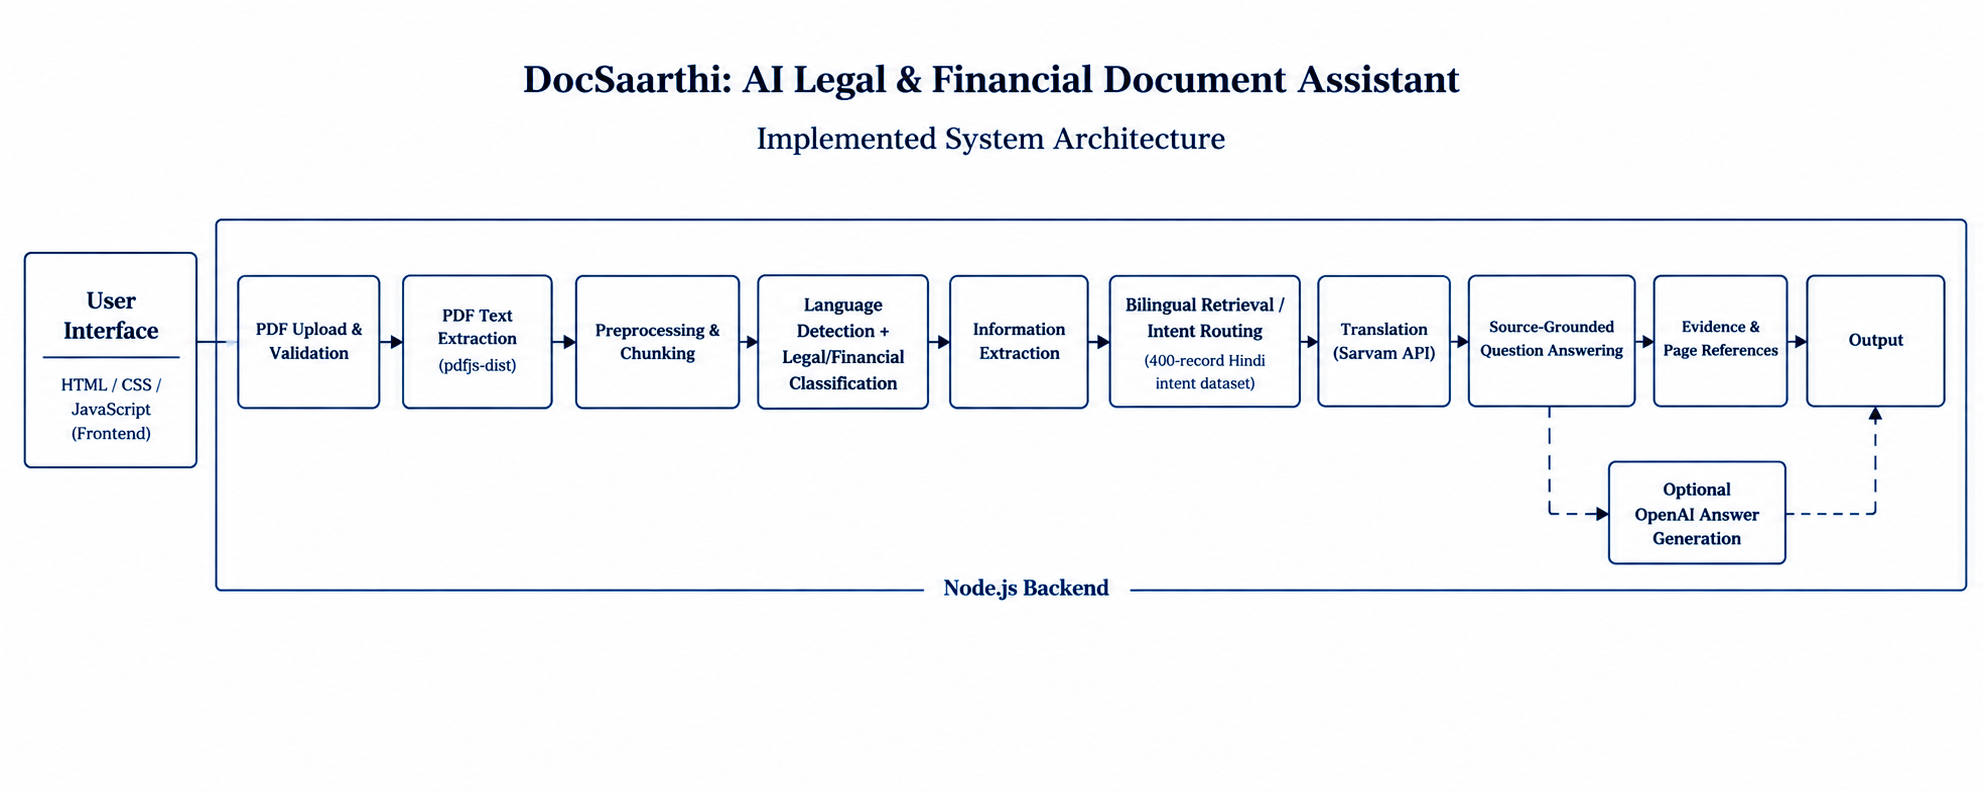
\includegraphics[width=0.95\textwidth]{figures/implemented_system_architecture.png.png}
\caption{Final Implemented System Architecture}
\label{fig:final_system_architecture}
\end{figure}

\section{Final End-to-End Workflow}
The user uploads a PDF; the server validates the file, extracts page-level text, detects language and document type, extracts important values, and builds searchable chunks. A user question is normalized and routed, relevant chunks are retrieved, an answer is formed only from those chunks, and the response includes page-linked evidence. Translation is performed on demand while the original PDF remains authoritative.

\section{Final System Implementation}
The implementation uses HTML, CSS, and JavaScript on the frontend; Node.js and Express on the backend; \texttt{pdfjs-dist} for extraction; local rule and lexical services for analysis and retrieval; and a 400-record Hindi dataset for intent signals. An offline English-Hindi parallel dataset supports known translations. OpenAI use is optional and controlled through configuration.

\section{Final Results}
The final build passes all 18 automated tests. On the eight-document labelled holdout, the system correctly classified all documents and detected both English and Hindi correctly. Source citations, page numbers, abstention, and critical-value preservation also passed their regression checks.

\section{Sample Outputs}
\begin{longtable}{|p{3.4cm}|p{4.3cm}|p{5.7cm}|}
\hline
\textbf{Input Scenario} & \textbf{Expected System Behavior} & \textbf{Verified Output Characteristic} \\
\hline
Hindi legal agreement with English termination query & Retrieve Hindi termination clause & Evidence contains the thirty-day clause and page 7 reference \\
\hline
English financial document with Hindi EMI query & Retrieve English repayment clause and answer in Hindi & Answer preserves the monthly EMI of ₹20,000 and cites the source excerpt \\
\hline
Question asking for absent PAN number & Do not infer an identifier & ``Information not found'' response, no source citation, grounded flag false \\
\hline
Financial translation request & Preserve protected values & Name, ₹5,00,000, 9.50\%, and 05/08/2029 remain unchanged \\
\hline
\end{longtable}

\section{Results Discussion}
The results show that a lightweight pipeline can provide useful, traceable assistance for controlled legal and financial samples. The strongest outcome is not the small-sample accuracy alone, but the combination of cross-language retrieval, source citations, value preservation, and safe abstention.

\section{Achievement of Project Objectives}
The prototype satisfies the principal objectives: PDF processing, Legal/Financial classification, bilingual interaction, structured information extraction, question answering from document evidence, page-level verification, and an accessible web interface. It also separates supporting datasets from authoritative document evidence.

\section{Limitations of the Final System}
The system does not yet support scanned PDFs without OCR, persistent multi-user storage, authentication, calibrated confidence, exhaustive legal or financial terminology, or production-scale evaluation. The translation memory can translate only supported content, and the in-memory repository loses documents when the server restarts.

\section*{Chapter Summary}
DocSaarthi delivers an operational end-to-end prototype with verified bilingual and grounding safeguards. The final results support academic demonstration while leaving clear work for production readiness.
